\subsection{Teilaufgabe 1: Algorithmik}

\subsection{Teilaufgabe 2: Theoretische Informatik}

\subsubsection{Aufgabe 1: Reguläre Sprachen}

\begin{teile}
	\item
	$L=(a|b|c)^*b(a|c)(c|ba)^*$		
	
	\item
	\underline{Schritt 1:} Umwandlung des NEA zum DEA mittels Potenzmengenkonstruktion:
	
	\begin{tabular}{c|c|c|c|c|l}
		\textbf{Zustand} & \textbf{Eingabe a} & \textbf{Eingabe b} & \textbf{Eingabe c} & \textbf{Final} & \textbf{Anmerkung} \\
		\hline
		q                & q                  & qr                 & q                  &                   & Neuer Zustand qr \\
		\hline
		qr               & qs                 & q                  & qs                 &                   & Neuer Zustand qs \\
		\hline
		qs               & q                  & qt                 & qs                 &  $\checkmark$                 & Neuer Zustand qt\\
		\hline
		qt               & qs                 & q                  & q                 &                   & \\
		\hline
	\end{tabular}
	
	Der Tabelle können aus der ersten Spalte die für den DEA benötigten Zustände entnommen werden. Zudem werden die Übergänge nach Eingabe von $a$, $b$ oder $c$ aufgeführt und die Endzustände gekennzeichnet.
	
	\underline{Schritt 2:} Der gesuchte DEA soll aber nicht $L$, sondern das Komplement von $L$ erkennen. Um das zu erreichen, werden Endzustände und Nicht-Endzustände vertauscht. Hier die graphische Darstellung des gesuchten DEA, der $\overline{L}$ akzeptiert:
	
	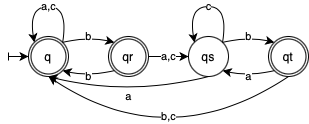
\includegraphics[scale=0.8]{Komplement-DEA}
		
	\item
	\underline{Schritt 1:} Angabe einer Zeugentabelle zur Überprüfung der Erreichbarkeit:

	\begin{tabular}{l|ccccccc}
		\textbf{Zustand} & q & r  & s          & t & x  & y & z \\
		\hline
		\textbf{Zeuge}   & 1 & 11 & $\epsilon$ & - & 01 & 0 & 00 \\
	\end{tabular} 
	
	Der Zustand t ist also nicht erreichbar und entfällt im minimierten Automaten.
	
	\underline{Schritt 2:} Identifizieren nicht äquivalenter Zustände über Tabelle mit Zustandspaaren:
	
	\includegraphics[scale=0.6]{Tabellenfüllverfahren.png}

	\textbf{Tabellenfüllverfahren} \\
	Zunächst werden alle Zustandspaare, die aus einem Endzustand und einem Nicht-Endzustand bestehen, mit X0 markiert. Weitere Kreuze in der Tabelle findet man mittels folgender Übergangstabelle von Zustandspaaren:

	\begin{tabular}{c|c|c|l}
		\textbf{Zustandspaar} & \textbf{0} & \textbf{1} & \textbf{Erläuterung} \\
		\hline
		(s,r)                 & (y,q)      & (q,x)      & Eingabe 0 führt mit (y,q) zu X0. Ergänze X1. \\
		\hline
		(x,r)                 & (r,q)      & (z,x)      & Eingabe 0 führt mit (r,q) zu X0. Ergänze X2. \\
		\hline
		(x,s)                 & (r,y)      & (z,q)      & Eingabe 1 führt mit (z,q) zu X0. Ergänze X3. \\
		\hline
		(y,s)                 & (z,y)      & (x,q)      & Eingabe 1 führt mit (z,q) zu X0. Ergänze X4. \\
		\hline
		(y,x)                 & (z,r)      & (z,x)      & Eingabe 1 führt mit (z,x) zu X0. Ergänze X5. \\
		\hline
		(z,q)                 & (x,x)      & (y,r)      & z und q sind äquivalent. \\
		\hline 		
		(y,r)                 & (z,q)      & (x,x)      & y und r sind äquivalent. \\
	\end{tabular} 
	
	Die Zustände $z$ und $q$ sowie $y$ und $r$ sind äquivalent, da auch bei wiederholter Überprüfung keine Übergänge gefunden werden, die zu einem Kreuz führen. Damit ergeben sich für den minimierten Automaten folgende Zustände, die den Äquivalenzklassen der Zustände von $A$ entsprechen: $[z,q],[y,r],[s],[x]$
	
	Der minimierte Automat A' lautet also: \\
	$A' = (\{[q,z],[y,r],[s],[x]\},\{0,1\},\delta',[s],\{[q,z]\})$ mit

	\begin{tabular}{c|c|c}
		$\delta'$ & 0 & 1 \\
		\hline
		[s]       & [y,r]      & [q,z] 	\\
		\hline
		[x]       & [y,r]      & [q,z]	\\
		\hline
		[y,r]     & [q,z]      & [x]	\\
		\hline
		[q,z]     & [x]        & [y,r]	\\
	\end{tabular}
\end{teile}

\newpage
\subsubsection{Aufgabe 2: Kontextfreie Sprachen}

\begin{teile}
	\item
	$G=(\{S,A,B\},\Sigma,P,S)$ mit $P$:\\
	\begin{tabular}{lcl}
		$S$ & $\rightarrow$ & $AB$ $\mid$ $\epsilon$ \\
		$A$ & $\rightarrow$ & $0A1 \mid 2A \mid \epsilon$ \\
		$B$ & $\rightarrow$ & $1B2 \mid B0 \mid \epsilon$ \\
	\end{tabular}
	
	\textbf{Konstruktionsidee} \\
	Im Kern beruht diese Grammatik auf der Idee, dass jedes Wort in $L$ aus zwei Teilwörtern besteht:
	\begin{itemize}
		\item
		einem linken Teilwort $x$, dass an seinem rechten Rand (also dem Mittelteil des Gesamtwortes) so viele 1en aufweist	wie es selbst 0en enthält, wobei links und rechts aller 0en beliebig viele 2en zulässig sind, und analog dazu
		\item
		einem rechten Teilwort $y$, dass an seinem linken Rand (also dem Mittelteil des Gesamtwortes) so viele 1en aufweist wie es selbst 2en enthält, wobei links und rechts der 2en beliebig viele 0en zulässig sind.			
	\end{itemize}

	Somit können $x$ und $y$ aus den Variablen $A$ und $B$ der Grammatik erzeugt werden und es ist jederzeit sichergestellt, dass im Gesamtwort $n = |w|_0 + |v|_2$ gilt, denn n entspricht der Summe der 1en in $x$ und $y$.
	
	\item 
	\underline{Ableitung:} $\underline{S}\Rightarrow \underline{A}B\Rightarrow 2\underline{A}B\Rightarrow 20\underline{A}1B\Rightarrow 202\underline{A}1B\Rightarrow 2022\underline{A}1B\Rightarrow 20221\underline{B}\Rightarrow 20221\underline{B}0\Rightarrow 202211\underline{B}20\Rightarrow 202211\underline{B}020\Rightarrow 2022111\underline{B}2020\Rightarrow 20221112020$
	
	\underline{Ableitungsbaum:}

	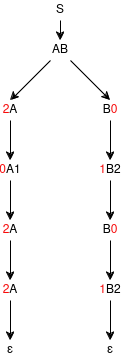
\includegraphics[scale=0.8]{Ableitungsbaum}
	
	\item
	$L = \{w1^n v \mid n \in \mathbb{N}, w, v \in \{0,2\}^*, n = |w|_0 \cdot |v|_2 \}$		
	
	\textbf{Beweis der Nicht-Kontextfreiheit}
	\begin{quote}
		\textbf{Pumpinglemma für kontextfreie Sprachen} \\
		Ist $L$ eine kontextfreie Sprache, so gilt: \\
		$\exists p \geq 1: \forall z \in L, |z| \geq p:$ \\
		$\exists u,v,w,x,y \in \Sigma^*: z = uvwxy$ mit
		\begin{enumerate}
			\item $|vx| \geq 1$
			\item $|vwx| \leq p$
			\item $\forall i \in \mathbb{N} : uv^{i}wx^{i}y \in L$
		\end{enumerate}
	\end{quote}
  	
	Nehmen wir an $L$ sei kontextfrei, dann können wir das Pumpinglemma anwenden und folgern:

	Sei $p \in \mathbb{N}$ die Pumpingzahl. Wir wählen $z = 0^p1^{p^2}2^p \in L$ mit $|z|=2p+p^2\geq p$.\\
	Aus $1$ und $2$ folgt: $vwx$ kann nicht aus $0$en, $1$en und $2$en bestehen und $vx$ darf nicht leer sein. Die Formen von $v$ und $x$ entsprechen also einem der vier Fälle (mit $1 \leq k+l+m \leq p$):
	\begin{itemize}
		\item Fall 1.1: $v=0^k1^l$ und $x=1^m$
		\item Fall 1.2: $v=0^k$ und $x=0^l1^m$
		\item Fall 2.1: $v=1^k2^l$ und $x=2^m$
		\item Fall 2.2: $v=1^k$ und $x=1^l2^m$
	\end{itemize}

	\underline{Fall 1.1:}\\
	Man erhält durch pumpen mit $i = 2$ das Wort $z'=uv^2wx^2y=0^{p+2k}1^{p^2+2(l+m)}2^{p}$.\\
	Angenommen $k\geq 1$. Damit $z' \in L$ gilt, muss $l+m = k*p$ und somit $k+l+m=k*(p+1)>p$ gelten. $\mbox{\Lightning}$\\
	Folglich muss $k=0$ sein. Aber es muss wieder $l+m = k*p = 0$ gelten und somit $k+l+m=0$. $\mbox{\Lightning}$

	\underline{Fall 1.2:}\\
	Man erhält durch pumpen mit $i = 2$ das Wort $z'=uv^2wx^2y=0^{p+2(k+l)}1^{p^2+2m}2^{p}$.\\
	Angenommen $k\geq 1$. Damit $z' \in L$ gilt, muss $m = (k+l)*p$ und somit $k+l+m=l*(p+1)+k*(p+1)>p$ gelten. $\mbox{\Lightning}$\\
	Folglich muss $k=0$ sein. Aber es muss wieder $m = (k+l)*p = l*p$ gelten.\\
	Ist nun $l\geq 1$ gilt $k+l+m=l*(p+1)>p$. $\mbox{\Lightning}$\\
	Falls aber $l=0$, ist auch $k+l+m=0$. $\mbox{\Lightning}$

	\underline{Fall 2.1:}\\
	Man erhält durch pumpen mit $i = 2$ das Wort $z'=uv^2wx^2y=0^{p}1^{p^2+2k}2^{p+2(l+m)}$.\\
	Angenommen $l\geq 1$. Damit $z' \in L$ gilt, muss $k = (l+m)*p$ und somit $k+l+m=l*(p+1)+m*(p+1)>p$ gelten. $\mbox{\Lightning}$\\
	Folglich muss $l=0$ sein. Aber es muss wieder $k = (l+m)*p = m*p$ gelten.\\
	Ist nun $m\geq 1$ gilt $k+l+m=m*(p+1)>p$. $\mbox{\Lightning}$\\
	Falls aber $m=0$, ist auch $k+l+m=0$. $\mbox{\Lightning}$

	\underline{Fall 2.2:}\\
	Man erhält durch pumpen mit $i = 2$ das Wort $z'=uv^2wx^2y=0^{p}1^{p^2+2(k+l)}2^{p+2m}$.\\
	Angenommen $m\geq 1$. Damit $z' \in L$ gilt, muss $k+l = m*p$ und somit $l+m+k=m*(p+1)>p$ gelten. $\mbox{\Lightning}$\\
	Folglich muss $m=0$ sein. Aber es muss wieder $k+l = m*p = 0$ gelten und somit $l+m+k=0$. $\mbox{\Lightning}$

	In jedem Fall ergibt sich ein Widerspruch zur Annahme $L$ sei kontextfrei. $\Rightarrow L$ ist nicht kontextfrei.
		
\end{teile}

\newpage
\subsubsection{Aufgabe 3: Entscheidbarkeit}
\begin{teile}
	\item
	Formulierung des Entscheidungsproblems als Wortproblem von\\
	$L=\{c(M)|\ M\ ist\ TM \wedge (\forall n \leq 42: \exists w \in \Sigma^*: |w|=n \wedge w \in L(M))\}$

	Hier soll nicht die Entscheidbarkeit widerlegt, sondern die Semientscheidbarkeit bewiesen werden. Daher wird nicht \textit{von einem Problem reduziert}, sondern stattdessen \textit{ein Entscheidungsverfahren aufgezeigt}.
	
	Dazu wird eine \textit{nichtdeterministische 3-Band} TM $M'$ skizziert, die alle $w \in L$ akzeptiert:
	\begin{enumerate}
		\item Syntaxcheck, ob $w=c(M)$ mit TM $M$, auf Band 1
		\item Simulieren von $M$ mit Eingabe $\varepsilon$ auf Band 2: Falls $M$ hält und akzeptiert, fortfahren mit Schritt 3; ansonsten halten und nicht akzeptieren
		\item Nichtdeterministische Auswahl eines Buchstaben $x_i \in \Sigma$ und Schreiben von $x_i$ auf Band 2, Zeiger eins nach rechts setzen
		\item $n$-maliges Wiederholen von Schritt 2, beginnen mit $n=1$ auf Band 3
		\item Simulieren von $M$ mit Eingabe $x_1x_2...x_n$ auf Band 2 (Zeiger dafür zuerst auf $x_1$ setzen): Falls $M$ hält und akzeptiert, fortfahren mit Schritt 6; ansonsten halten und nicht akzeptieren
		\item $n$ um eins erhöhen auf Band 3 und solange $n \leq 42$ zu Schritt 4 zurückspringen: Falls $n > 42$ halten und akzeptieren
	\end{enumerate}

	\underline{Anmerkungen zu $M'$:} Da DTM und NTM, sowie Einband- und Mehrband-Maschinen gleich mächtig sind, spielt es keine Rolle welche Anzahl an Bändern und welchen Typ von Maschine man hier wählt. Die \textit{nichtdeterministische} Funktionsweise von $M'$ stellt sicher, dass die in Schritt 3 stückweise "geratenen“ Wörter immer genau diejenigen von Länge $n$ sind, welche in $L(M)$ liegen (Vorstellung vom allwissenden Orakel).

	Die TM $M'$ akzeptiert alle $w \in L$, somit ist $L$ semi-entscheidbar.
	
	\vspace{0.3cm}

	\item
	\begin{quote}	
		\textbf{Satz von Rice (für formale Sprachen)}\\
		Sei $\mathcal{S} $ eine nicht leere, echte Teilmenge der Menge aller formalen Sprachen.\\
		Dann ist die folgende formale Sprache unentscheidbar:\\
		$L_\mathcal{S}  = \{c(M) |\ M\ ist\ TM\ und\ L(M)\ liegt\ in\ \mathcal{S}\}$
	\end{quote}
	
	\underline{Umschreiben von $L$:}\\
	$L=\{c(M)|\ M\ ist\ TM \wedge L(M) \in \mathcal{S}$ mit $\mathcal{S} := \{L\subseteq \Sigma^* | \forall n \leq 42: \exists w \in \Sigma^*: |w|=n \wedge w \in L\}$

	\underline{Nachweis der Nichttrivialität der Menge $\mathcal{S}$:}

	$\Sigma^* \in \mathcal{S}$, da in $\Sigma^*$ Worte mit beliebiger Länge liegen $\Rightarrow \mathcal{S} \neq \varnothing$.

	$\{\varepsilon\} \notin \mathcal{S}$, da in $\{\varepsilon\}$ z.B. kein Wort der Länge 3 liegt $\Rightarrow \mathcal{S}$ ist nicht die Menge aller formalen Sprachen.

	Somit folgt nach dem Satz von Rice, dass $L$ nicht entscheidbar ist.

\end{teile}

\newpage
\subsubsection{Aufgabe 4: NP-Vollständigkeit}

\begin{teile}
	\item 
	Dazu wird das Vorgehen einer nichtdeterministischen Zweiband-TM skizziert, welche das Problem im Polynomieller Zeit lößt:
	\begin{enumerate}
		\item Überprüfe, ob $w$ von der Form $c(V,E,k)$ ist mit $(V,E)$ repräsentiert einen Graphen $G$ und $k \in \mathbb{N}$ (auf Band 1).
		\item Wähle nichtdeterministisch einen Knoten $v'$ aus $V$ und füge ihn der Knotenmenge $V'$ hinzu (kodiert auf Band 2).
		\item Überprüfe, ob es zu $v'$ ein $v''$ in $V'$ gibt, sodass $(v',v'')\in E$ liegt (auf Band 2). \begin{itemize}
			\item Falls es kein solches $v''$ in $V'$ gibt, wiederhole ab Schritt 2.
			\item Falls genau ein solches $v''$ in $V'$ existiert und $|V'|\geq k$ gilt, halte und akzeptiere.
			\item Falls mehrere Kandidaten für $v''$ in $V'$ gefunden werden und $|V'|-1\geq k$ gilt, halte und akzeptiere.
			\item Falls mehrere Kandidaten für $v''$ in $V'$ gefunden werden und $|V'|-1 < k$ gilt, halte und akzeptiere \underline{nicht}.
		\end{itemize}
	\end{enumerate}
	\textit{Anmerkung: Durch die nichtdeterministische Wahl wird stets das passende $v'$ hinzugefügt, falls ein solches existiert (Vorstellung vom allwissenden Orakel).}

	\textbf{Laufzeitanalyse:} Der Syntaxcheck in Schritt 1 läut mit nichtdeterministischem Raten der Übergänge im Eingabewort von $V$ nach $E$ und nach $k$ in $O(|V|)+O(|E|)+O(k)\leq O(n)$. Schritt 2 läuft maximal in $O(|V'|)\leq O(|V|)\leq O(n)$. Die erste Überprüfung in Schritt 3 erfordert höchstens $O(|V'|)\cdot O(|E|)\leq O(n^2)$. Die Bestimmung der Mächtigkeit von $V'$ und der Abgleich mit $k$ erfolgen in $O(|V'|)+O(k)\leq O(n)$.\\
	Die Schritte 2 und 3 werden höchstens $|V|$ mal wiederholt. Insgesamt arbeitet die NTM also in $O(n^3)$.

	Daraus folgt, dass das in der Aufgabe beschriebene Graphenproblem in NP liegt.

	\item
	Sei	$L_1=\{c(V,E,k)\ |\ G=(V,E)\ ist\ Graph \wedge k\in \mathbb{N}: \exists V' \subseteq V:(\nexists e=(v_1,v_2)\in E\ mit\ v_1,v_2 \in V') \wedge |V'|\geq k \}$\\
	die Sprache, deren Wortproblem gleich dem Entscheidungsproblem einer unabhängigen Menge in $G$ ist.

	Sei	$L_2=\{c(V,E,k)\ |\ G=(V,E)\ ist\ Graph \wedge k\in \mathbb{N}: \exists V' \subseteq V:|\{e=(v_1,v_2)\in E\ |\ v_1,v_2 \in V'\}|\leq 1 \wedge |V'|\geq k \}$\\
	die Sprache, deren Wortproblem gleich dem Entscheidungsproblem einer fast unabhängigen Menge mit mindestens $k$ Knoten in $G$ ist.

	Man verwende folgenden Ansatz für die polynomielle Reduktion:\\
	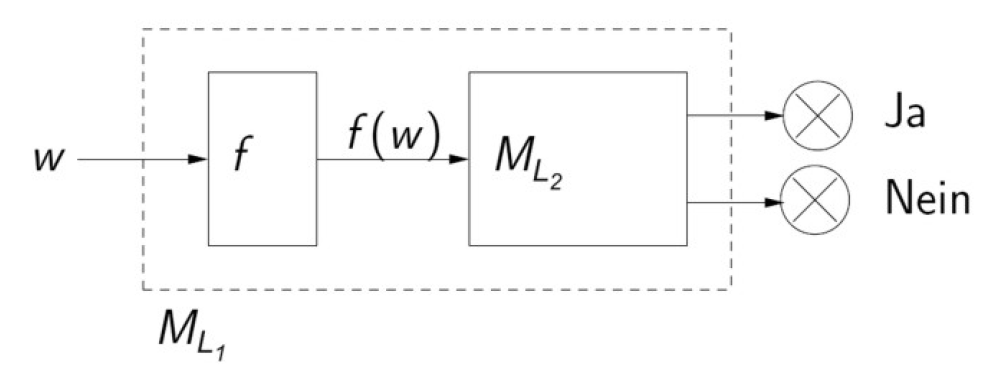
\includegraphics[scale=0.4]{reduction_idee_skizze}

	Dazu wird eine totale und berechenbare Funktion $f$ benötigt, die das Wortproblem aus $L_1$ auf das Wortprobleme aus $L_2$ abbildet:

	Sei $f:L_1 \rightarrow L_2$ definiert über

	$f(w)=\begin{cases}
		c(\tilde{V},\tilde{E},\tilde{k})&\text{falls $w=c(V,E,k)$ mit $G=(V,E)$ ist Graph und $k \in \mathbb{N}$}\\
		\varepsilon &\text{sonst}
	\end{cases}$\\
	Dabei wird $V$ um zwei Knoten $v_1,v_2 \notin V$ ergänzt und zum neuen $\tilde{V}=V\cup \{v_1,v_2\}$. Die neuen Knoten bilden auch eine Kante, somit ist $\tilde{G}=G\cup \{(v_1,v_2)\}$. Außerdem gilt $\tilde{k}=k+2$.

	$f$ ist offensichtlich total. Außerdem lässt sich eine DTM konstruieren, die $f$ in polynomieller Laufzeit berechnet:
	\begin{itemize}
		\item Syntaxcheck, ob $w$ von der Form $c(V,E,k)$ ist, wobei $(V,E)$ einen Graphen $G$ repräsentiert und $k \in \mathbb{N}$ (höchstens in $O(n^2)$).
		\item An die Kodierung von $V$ zwei neue Knoten $v_1$ und $v_2$ anhängen (höchstens in $O(n^2)$).
		\item An die Kodierung von $G$ die neue Kante $(v_1,v_2)$ anhängen (höchstens in $O(n)$).
		\item Zu $k$ in der entsprechenden Kodierung $2$ addieren (höchstens in $O(n)$).
	\end{itemize}

	Es bleibt noch zu zeigen, dass $w \in L_1 \Leftrightarrow f(w) \in L_2$ gilt. Dies beweisen folgende Äquivalenzumformungen ($\forall w \in L_1$):
	\begin{align*}
		w \in L_1 \Leftrightarrow\ & w=c(V,E,k)\ mit\ G=(V,E)\ ist\ Graph\ und\ k \in \mathbb{N}\\
		& \wedge (\exists V'\subseteq V:\nexists e=(v_1,v_2)\in E\ mit\ v_1,v_2 \in V' \wedge |V'|\geq k)\\
		\Leftrightarrow\ &f(w)=c(\tilde{V},\tilde{E},\tilde{k})\ mit\ \tilde{G}=(\tilde{V},\tilde{E})\ ist\ Graph\ und\ \tilde{k} \in \mathbb{N}\\
		& \wedge (\exists V'\subseteq V:\nexists e=(v_1,v_2)\in E\ mit\ v_1,v_2 \in V' \wedge |V'|\geq \tilde{k}-2)\\
		\Leftrightarrow\ &f(w)=c(\tilde{V},\tilde{E},\tilde{k})\ mit\ \tilde{G}=(\tilde{V},\tilde{E})\ ist\ Graph\ und\ \tilde{k} \in \mathbb{N}\\
		& \wedge (\exists \tilde{V'}\subseteq \tilde{V}:\exists! e=(v_1,v_2)\in \tilde{E}\ mit\ v_1,v_2 \in \tilde{V'} \wedge |\tilde{V'}|=|V'|+2\geq \tilde{k})\\
		\Leftrightarrow\ &f(w)=c(\tilde{V},\tilde{E},\tilde{k})\ mit\ \tilde{G}=(\tilde{V},\tilde{E})\ ist\ Graph\ und\ \tilde{k} \in \mathbb{N}\\
		& \wedge (\exists \tilde{V'}\subseteq \tilde{V}: |\{e=(v_1,v_2)\in \tilde{E}\ \vert\ v_1,v_2 \in \tilde{V'}\}|\leq 1 \wedge |\tilde{V'}|\geq \tilde{k})\\
		\Leftrightarrow\ &f(w) \in L_2
	\end{align*}
	\textit{Informelle Beschreibung: Man füge zwei neue Knoten mit einer gemeinsamen Kante hinzu und erhöhe $k$ um $2$. Somit kann für jede unabhängige Menge in $L_1$ mit Mächtigkeit $k$ eine fast unabhängige Menge in $L_2$ mit Mächtigkeit $k+2$ gefunden werden, die zusätzlich genau die neu hinzugefügten Knoten enthält. Falls eine fast unabhängige Menge in $L_2$ nur einen der extra hinzugefügten Knoten enthält, muss eine Kante aus $E$ enthalten sein. Allerdings kann dann einer der Knoten dieser Kante weggelassen werden und es gibt immer noch eine unabhängige Menge in $L_1$ mit zwei Knoten weniger (einer der hinzugefügten und einer aus der Kante). Die Rückrichtung stimmt also auch.}

	Somit gilt $L_1 \leq_p L_2$ und da $L_1$ NP-hart ist, muss $L_2$ auch NP-hart sein, denn die Relation $\leq_p$ ist transitiv. Da $L_2$ zudem in NP liegt (siehe (a)), ist $L_2$ und damit das entsprechende Graphenproblem NP-vollständig.
	
\end{teile}

\newpage
\subsubsection{Aufgabe 5: Aussagen}
\begin{teile}
	\item
	Falsch.\\
	Unabhängig von $\Sigma$ kann $L=\{\varepsilon \}$ gewählt werden. Diese Sprache wird offensichtlich durch eine DTM entschieden, die auf der leeren Eingabe hält und akzeptiert und bei nicht leerer Eingabe hält und nicht akzeptiert.
	
	\item
	Falsch.\\
	Betrachte die Sprache $L=\{a^n \vert n\in \mathbb{P}\cup \{0,1\}\}$, welche wegen der Primzahleigenschaften bekanntermaßen nicht regulär ist. Allerdings ist $L^*=\{a^n \vert n\in \{\sum_{i = 0}^{\infty} a_i \vert a_i \in \mathbb{P}\cup \{0,1\}\}\}=\{a^n \vert n\in \mathbb{N}_0\}=\Sigma^*$, da alle $n \in \mathbb{N}$ als Summe von $1$en dargestellt werden können. $L^*=\Sigma^*$ ist allerdings trivialer Weise regulär.
	
	\item
	Richtig.\\
	\textit{Beweis durch Widerspruch:} Sei $L$ unentscheidbar. Wir nehmen an, dass $\overline{L} \in \mathcal{NP}$. Demnach gibt es eine NTM $M$, die $\overline{L}$ in polynomieller Zeit akzeptiert. %Also gibt es auch eine DTM $M'$, die $\overline{L}$ in exponentieller Zeit akzeptiert. Darüber kann eine DTM $\overline{M'}$ konstruiert werden, welche $M'$ simuliert und lediglich akzeptieren und nicht-akzeptieren vertauscht und somit $L$ entscheidet. $\mbox{\Lightning}$\\
	Darüber kann eine NTM $M'$ konstruiert werden, welche $M$ simuliert und lediglich akzeptieren und nicht-akzeptieren vertauscht. Da $M$ in polynomieller Zeit arbeitet, tut dies auch $M'$ und entscheidet somit $L$. $\mbox{\Lightning}$\\
	$\Rightarrow$ Wenn $L$ unentscheidbar ist, muss $\overline{L} \notin \mathcal{NP}$ gelten.

	\item
	Richtig.\\
	Da die DTM $M$ jedes Eingabewort in konstanter Zeit entscheidet, kann ein DEA konstruiert werden, der $M$ simuliert und so $L$ akzeptiert. Dafür sind höchstens $k\cdot 3\cdot(|\Sigma|+1)\cdot |\Gamma|$ - also endlich viele - Zustände nötig (maximal $k$ Berechnungsschritte mit $3$ möglichen Zeigerbewegungen, $|\Sigma|+1$ möglichen Eingabesymbolen bzw. einem leeren Übergang und $|\Gamma|$ möglichen Werten auf dem Band).\\
	Deshalb muss $L=L(M)$ regulär sein.
\end{teile}